\documentclass{article}
\usepackage{tikz}
\usepackage[margin=2cm]{geometry}

\begin{document}

\begin{center}
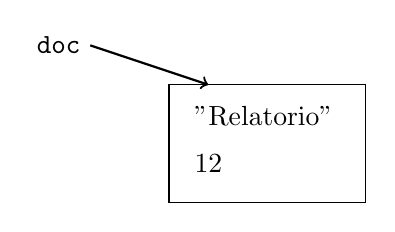
\begin{tikzpicture}

% Seta para o primeiro nó com rótulo "fila"
\draw[->, thick] (-1, 2) -- (0.5, 1.5);
\node[anchor=east] at (-1, 2) {\texttt{doc}};

% Nó 1
\draw (0, 0) rectangle (2.5, 1.5);
\node[anchor=west] at (0.2, 1.1) {"Relatorio"};
\node[anchor=west] at (0.2, 0.5) {12};


\end{tikzpicture}
\end{center}

\end{document}
